\chapter{角动量理论}
%%%%%%%%%%%%%%%%%%%%%%%%%%%%%%%%%%%%%%%%%%%%%%%%%%%
%%%%%%%%%%%%%%%%%%%%%%%%%%%%%%%%%%%%%%%%%%%%%%%%%%%

\section{角动量}
%%%%%%%%%%%%%%%%%%%%%%%%%%%%%%%%%%%%%%%%%%%%%%%%%%%
\paragraph*{角动量算符} 
量子力学中的角动量与经典中的类似,是一个三分量矢量,但在量子力学中需要考虑其满足的对易关系。把满足如下对易关系的三分量矢量称为角动量:
\begin{theorem}{角动量算符的充要条件}
	\begin{equation}
		J^{\dagger}_k = J_k, ~ k = 1, 2, 3, \quad \left[J_i, J_j\right] = i\hbar \sum_{k} \epsilon_{ijk} J_k
	\end{equation}
\end{theorem}
其中,$\epsilon_{ijk}$是反对称的三维Levi-Civita排序符号。其有如下性质:a. 若有两个指标相同,则$\epsilon_{ijk} = 0$;b. 若三个指标两两不等,按循环排序,即如下图所示的排序时,有$\epsilon_{123} = \epsilon_{231} = \epsilon_{312} = 0$;c. 剩下的排序将使排序符号为$-1$;用下标表示$1 \equiv x$、$2 \equiv y$和$3 \equiv z$。
\begin{figure}[htbp]
	\centering
	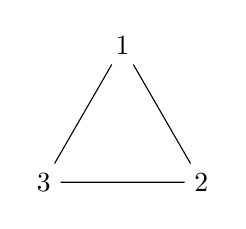
\begin{tikzpicture}
		\node (A) at (0,0) {3};
		\node (B) at (2,0) {2};
		\node (C) at (60:2) {1};
		\draw (A) -- (B) -- (C) -- (A);
	\end{tikzpicture}
\end{figure}

\paragraph*{角动量算符的本征态和本征值} 角动量$\boldsymbol{J}$的本征态和本征值如下
\begin{align}
	\boldsymbol{J}^2 |j\ m\rangle =& j(j+1)\hbar^2 |j\ m\rangle	\\
	J_z |j\ m\rangle =& m\hbar |j\ m\rangle
\end{align}
其正交性和归一性为
\begin{equation}
	\langle j^{\prime}\ m^{\prime} | j\ m\rangle = \delta_{jj^{\prime}}\delta_{mm^{\prime}}, \quad m = -j,\ -j+1, \ \cdots, j-1,\ j \ .
\end{equation}
此外,我们定义角动量的梯度算符
\begin{equation}
	J_{\pm} = J_{x} \pm i J_{y}
\end{equation}
满足对易式
\begin{equation}
	\left[J_{+}, J_{-}\right] = 2\hbar J_z, \quad \left[J_{\pm}, J_{z}\right] = \mp \hbar J_{\pm}
\end{equation}
梯度算符作用到本征态上的效果为
\begin{equation}
	\begin{aligned}
		J_{\pm} |j\ m\rangle =& \hbar \sqrt{j(j+1) - m(m\pm)1} |j\ m\pm 1\rangle	\\
						   =& \hbar \sqrt{(j\pm m +1) (j\mp m)} |j\ m\pm 1\rangle
	\end{aligned}
\end{equation}
对于单粒子在希尔伯特空间中的抽象角动量本征态$|j\ m\rangle$的坐标表示通常为\underline{球谐函数}。

%%%%%%%%%%%%%%%%%%%%%%%%%%%%%%%%%%%%%%%%%%%%%%%%%%%
%%%%%%%%%%%%%%%%%%%%%%%%%%%%%%%%%%%%%%%%%%%%%%%%%%%
\section{两角动量耦合与CG系数}
考虑两个完全对易的角动量$\boldsymbol{J}_1$和$\boldsymbol{J}_2$,也就是说这两个角动量分别属于两个不同的粒子,或者是一个粒子的自旋角动量和轨道角动量间的耦合。用CG系数表示耦合前和耦合后的角动量间关系。对于这样的两个角动量,我们有关系成立
\begin{equation}
	\left[\bmJ_1, \bmJ_2 \right] = 0 \quad
	\text{or}
	\quad
	\left[J_{1k}, J_{2l}\right] = 0,\ \text{for all}\ k, l = 1, 2, 3
\end{equation}

\paragraph*{CG系数} CG系数的解析表达式如下[\textit{Quantum Theory of Angular Momentum}, Eq. 8.2.1(3)]
\begin{equation}
    \begin{aligned}
        C_{j_1 m_1 j_2 m_2}^{j_3 m_3} 
        &= \delta_{m_3, m_1 + m_2} \Delta(j_1 j_2 j_3) \\
        \times& \left[ (j_1 + m_1)! (j_1 - m_1)! (j_2 + m_2)! (j_2 - m_2)! 
                 (j_3 + m_3)! (j_3 - m_3)!(2j_3 + 1)\right]^{1/2} \\
            \times& \sum_{k}\left[\frac{(-1)^k}{k!(j_1 + j_2 - j_3 - k)!(j_1 - m_1 - k)!
            (j_2 + m_2 - k)!(j_3 - j_2 + m_1 +k)!}\right.\\
                  &\left. \cdot \frac{1}{(j_3 - j_1 - m_2 + k)!} \right]
    \end{aligned}
    \label{eq:CG-representations}
\end{equation}
上式的$\Delta-symbol$定义如下
\begin{equation*}
    \Delta(j_1 j_2 j_3) = \left[ \frac{(j_1 + j_2 - j_3)! (j_1 - j_2 + j_3)! (-j_1 + j_2 + j_3)!}
                                      {(j_1 + j_2 + j_3 +1)!} \right]^{\frac{1}{2}}
\end{equation*}
其中,求和的上下限需保证所有阶乘项的自变量为非负,应满足一下条件
\begin{equation}
    \begin{aligned}
        k_{min} = \text{max} \left\{ 0, j_2 - m_1 - j_3, j_1 + m_2 - j_3 \right\}\\
        k_{max} = \text{min} \left\{ j_1 + j_2 - j_3, j_1 - m_1, j_2 + m_2 \right\}
    \end{aligned}
    \label{eq:CG-nonnegative}
\end{equation}



%%%%%%%%%%%%%%%%%%%%%%%%%%%%%%%%%%%%%%%%%%%%%%%%%%%
